%%%%%%%%%%%%%%%%%%%%%%%%%%%%%%%%%%%%%%%%%
% Beamer Presentation
% LaTeX Template
% Version 1.0 (10/11/12)
%
% This template has been downloaded from:
% http://www.LaTeXTemplates.com
%
% License:
% CC BY-NC-SA 3.0 (http://creativecommons.org/licenses/by-nc-sa/3.0/)
%
%%%%%%%%%%%%%%%%%%%%%%%%%%%%%%%%%%%%%%%%%

%----------------------------------------------------------------------------------------
%	PACKAGES AND THEMES
%----------------------------------------------------------------------------------------

\documentclass[aspectratio=169]{beamer}
\usefonttheme[onlymath]{serif} % Makes it looks like proper maths
\mode<presentation> {

    % The Beamer class comes with a number of default slide themes
    % which change the colors and layouts of slides. Below this is a list
    % of all the themes, uncomment each in turn to see what they look like.

    %\usetheme{default}
    %\usetheme{AnnArbor}
    \usetheme{Antibes}
    %\usetheme{Bergen}
    %\usetheme{Berkeley}
    %\usetheme{Berlin}
    %\usetheme{Boadilla}
    %\usetheme{CambridgeUS}
    %\usetheme{Copenhagen}
    %\usetheme{Darmstadt}
    %\usetheme{Dresden}
    %\usetheme{Frankfurt}
    %\usetheme{Goettingen}
    %\usetheme{Hannover}
    %\usetheme{Ilmenau}
    %\usetheme{JuanLesPins}
    %\usetheme{Luebeck}
    %\usetheme{Madrid}
    % \usetheme{Malmoe}
    %\usetheme{Marburg}
    %\usetheme{Montpellier}
    %\usetheme{PaloAlto}
    %\usetheme{Pittsburgh}
    %\usetheme{Rochester}
    %\usetheme{Singapore}
    %\usetheme{Szeged}
    %\usetheme{Warsaw}

    % As well as themes, the Beamer class has a number of color themes
    % for any slide theme. Uncomment each of these in turn to see how it
    % changes the colors of your current slide theme.

    %\usecolortheme{albatross}
    %\usecolortheme{beaver}
    %\usecolortheme{beetle}
    %\usecolortheme{crane}
    %\usecolortheme{dolphin}
    %\usecolortheme{dove}
    %\usecolortheme{fly}
    %\usecolortheme{lily}
    %\usecolortheme{orchid}
    %\usecolortheme{rose}
    %\usecolortheme{seagull}
    %\usecolortheme{seahorse}
    %\usecolortheme{whale}
    %\usecolortheme{wolverine}

    %\setbeamertemplate{footline} % To remove the footer line in all slides uncomment this line
    %\setbeamertemplate{footline}[page number] % To replace the footer line in all slides with a simple slide count uncomment this line
    \setbeamertemplate{navigation symbols}{} % To remove the navigation symbols from the bottom of all slides uncomment this line
}

\usepackage{graphicx} 
\usepackage{booktabs}
\usepackage{amsmath,amssymb}
\usepackage[authoryear,round]{natbib}
\usepackage{subfig}
\usepackage[]{color}
\newcommand{\bigCI}{\mathrel{\text{\scalebox{1.07}{$\perp\mkern-10mu\perp$}}}}
\definecolor{darkblue}{rgb}{0.0, 0.0, 0.55}
\definecolor{darkred}{RGB}{12, 144, 36}


%----------------------------------------------------------------------------------------
%	TITLE PAGE
%----------------------------------------------------------------------------------------

\title[Nonparametrics]{Bayesian nonparametric methods for dynamics identification and segmentation for powered
prosthesis control}

\author
{\texorpdfstring{
        Neil Dhir  \\
        \footnotesize 
        {\bf Machine Learning Research Group} [Osborne] \\
        {\bf Applied AI Laboratory} [Posner] \\
        (and Probabilistic Programming Group [Wood])
        \vspace{1cm}\\
        {Viva voce}
    }% 
    %\institute{Viva voce} % Your institution as it will appear on the bottom of every slide, may be shorthand to save space
    {} 
\date{\today}} % Date, can be changed to a custom date

\begin{document}

\begin{frame}[plain,noframenumbering]
    \titlepage % Print the title page as the first slide
\end{frame}

\begin{frame}[plain,noframenumbering]
    \frametitle{Overview} % Table of contents slide, comment this block out to remove it
    \tableofcontents % Throughout your presentation, if you choose to use \section{} and \subsection{} commands, these will automatically be printed on this slide as an overview of your presentation
\end{frame}

%----------------------------------------------------------------------------------------
%	PRESENTATION SLIDES
%----------------------------------------------------------------------------------------

\section{Motivation}

\begin{frame}[plain]
    \subsection{High-level}
    \frametitle{Motivation: high-level}
    \begin{columns}[t] % The "c" option specifies centered vertical alignment while the "t" option is used for top vertical alignment

        \column{.5\textwidth} % Left column and width
        \begin{itemize}
            \item Multiple-sclerosis: severely affects and reduces mobility 
            \item Diabetes: can give rise to complications e.g. heart disease, kidney disease
                retinopathy and neuropathy. 
            \item {\it Diabetes is the leading cause of amputation} 
            \item Quality of living through ability to perform activities of daily living such as locomotion
        \end{itemize}
        \column{.5\textwidth} % Right column and width
        \begin{figure}[ht]
            \includegraphics[width=.7\textwidth]{figures/parents.jpg}
            \caption{Parents}
        \end{figure}
    \end{columns}
\end{frame}

%------------------------------------------------

\begin{frame}[plain]
    \subsection{Mid-level}
    \frametitle{Motivation: mid-level}
    \begin{figure}
        \centering
        \includegraphics[width=0.9\textwidth]{figures/tucker.png}
        \caption{Generalised control framework for active prostheses and orthoses \citep{tucker2015control}.}
    \end{figure}
\end{frame}

%------------------------------------------------

\begin{frame}[plain,noframenumbering]
    \subsection{Low-level}
    \frametitle{Motivation: low-level}
    \begin{columns}[t] % The "c" option specifies centered vertical alignment while the "t" option is used for top vertical alignment
        \column{.5\textwidth} % Left column and width
        \begin{itemize}
            \item Perception layer 
                \begin{itemize}
                    \item {\bf Chapter III:} Incidence detection 
                    \item {\bf Chapter IV:} Dynamics identification via time-series segmentation
                \end{itemize}
            \item Translation/Execution layer 
                \begin{itemize}
                    \item {\bf Chapter V:} Gaussian process regression for prosthesis control 
                \end{itemize}
        \end{itemize}

        Three broad themes were addressed which fit into the control stratification proposed by
        \citet{tucker2015control}.

        \column{.5\textwidth} % Left column and width
        \begin{figure}[ht]
            \centering
            \includegraphics[width=.9\textwidth]{figures/half-tucker.png}
            \caption{Parts of a hierarchical controller \citep{tucker2015control}.}
        \end{figure}
    \end{columns}
\end{frame}

%------------------------------------------------

\section{Chapter III: Incidence detection [Perception layer]}
\begin{frame}[plain]
    %\subsection{High-level}
    \frametitle{Chapter III: Incidence detection [Perception layer]}
    \begin{columns}[t] 
        \column{.6\textwidth} % Left column and width
        \fbox{
            \begin{minipage}{7cm}
                The purpose of the high-level control is to perceive the locomotive intent of the user through 
                activity mode detection.
            \end{minipage}
        }
        \vspace{0.3cm}
        \begin{itemize}
            \item Use standard discriminative and generative approaches for classification 
            \item Demonstrate that popular original study by \citet{luvstrek2009fall} could be improved 
            \item Missing data was in-painted using a generative model (Kalman smoother)
            \item Dimensionality reduction operated upon complete data
            \item Increased performance was demonstrated with this simple approach
        \end{itemize}
        \column{.4\textwidth} % Right column and width
        \begin{figure}
            \vspace{-1.5cm}
            \centering
            \includegraphics[width=1.1\textwidth]{/home/nd/cloud/thesis/figures/walking-stick-man.pdf}
            \caption{Example of `walking' incidence \citep{dhir2014improved}.}
        \end{figure}
    \end{columns}
\end{frame}

%------------------------------------------------

\begin{frame}[plain,noframenumbering]
    \frametitle{Chapter III: Example observations}
    \begin{figure}
        \centering
        \includegraphics[width=0.9\textwidth]{/home/nd/cloud/thesis/figures/luvstrek-data-plot.pdf}
        \caption{Recordings made from an infrared motion capture system. Window shows marker
            trajectories of the coordinates of two (out of 12) markers attached to the bodies of three volunteers. The scenario depicted includes three activities, enacted in the following
        order: walking $\rightarrow$ falling $\rightarrow$ lying.}
    \end{figure}
\end{frame}

%------------------------------------------------

\begin{frame}[plain]
    %\subsection{High-level}
    \frametitle{Chapter III: Methods}
    \begin{columns}[t] 
        \column{.5\textwidth} % Left column and width
        \begin{figure}
            \centering
            \includegraphics[width=1\textwidth]{figures/kalman.png}
            \caption{Kalman smoothing to estimate trajectory; with \textcolor{green}{observations},
            \textcolor{red}{ground truth} and \textcolor{blue}{estimates} \citep{barber2012bayesian}.}
        \end{figure}
        \column{.5\textwidth} % Right column and width
        \begin{figure}
            \centering
            \includegraphics[width=.9\textwidth]{figures/MLDA.png}
            \caption{Multiclass linear discriminant analysis of a two-dimensional demonstration space
            \citep{Bishop:2006:PRM:1162264}.}
        \end{figure}
    \end{columns}
\end{frame}

%------------------------------------------------

\begin{frame}[plain]
    %\subsection{High-level}
    \frametitle{Chapter III: Results}
    \begin{columns}[t] 
        \column{.5\textwidth} % Left column and width
        \begin{figure}
            \centering
            \includegraphics[width=0.9\textwidth]{/home/nd/cloud/thesis/figures/raw_class_all.eps}
            \caption{Methods applied to raw data.}
        \end{figure}
        \column{.5\textwidth} % Right column and width
        \begin{figure}
            \centering
            \includegraphics[width=0.9\textwidth]{/home/nd/cloud/thesis/figures/dr_main.eps}
            \caption{Methods applied to feature vectors.}
        \end{figure}
    \end{columns}
\end{frame}

%------------------------------------------------

\begin{frame}[plain]
    %\subsection{High-level}
    \frametitle{Chapter III: Conclusions}
    \begin{columns}[t] 
        \column{.5\textwidth} % Left column and width
        \begin{itemize}
            \item Able to significantly improve {\bf supervised} classification performance using very simple, off-the-shelf, tools 
            \item In-painting proved valuable to complete the dataset
            \item Though complete, the dataset also has lots of redundancy, removed through dimensionality reduction
                (DR)
            \item DR was the primary driver of improved performance
            \item Additional experiments investigated information content of individual tags (see RHS figure)
        \end{itemize}
        \column{.5\textwidth} % Right column and width
        \begin{figure}
            \centering
            \includegraphics[width=.5\textwidth]{/home/nd/cloud/thesis/figures/foo2_updates2.eps}
            \caption{Illustration of activity, with best individual tag classification
            accuracy quoted with each tag \citep{dhir2014improved}.}
        \end{figure}
    \end{columns}
\end{frame}

%------------------------------------------------

\begin{frame}[plain]
    \frametitle{Reminder: Where are we now in the control hierarchy?}
    \begin{figure}
        \centering
        \includegraphics[width=0.9\textwidth]{figures/tucker.png}
        \caption{Generalised control framework for active prostheses and orthoses \citep{tucker2015control}.}
    \end{figure}
\end{frame}

%------------------------------------------------

\section{Chapter IV: Dynamics identification via time-series segmentation [Perception layer]}

\begin{frame}[plain]
    \frametitle{Chapter IV: Dynamics identification via time-series segmentation [Perception layer]}
    \begin{columns}[t] 
        \column{.5\textwidth} % Left column and width
        \fbox{
            \begin{minipage}{7cm}
                The purpose of the high-level control is to perceive the locomotive intent of the user through 
                activity mode detection.
            \end{minipage}
        }
        \begin{itemize}
            \item Traditional setting: supervised learning (Ch. III) using discriminative models
            \item Must consider unsupervised setting using generative modelling 
            \item Behaviours and activities are likely to grow with time, hence it is unsatisfactory to bound the
                state-space 
            \item Incidence detection and labelling must be {\bf automatic} 
        \end{itemize}
        \column{.5\textwidth} % Right column and width
        \begin{figure}
            \centering
            \includegraphics[width=.5\textwidth]{figures/state-seq-data1.pdf}
            \includegraphics[width=.5\textwidth]{figures/state-seq-data2.pdf}
            \caption{Unsupervised learning of slow and fast dynamics.}
        \end{figure}
    \end{columns}
\end{frame}

%------------------------------------------------

\begin{frame}[plain,noframenumbering]
    \frametitle{Chapter IV: Generative sequence modelling}
    \begin{itemize}
        \item Time-series labelling is laborious and subjective $\rightarrow$ use semi/un-supervised learning to support labelling exercise
        \item Want to discover new behaviours $\rightarrow$ Bayesian nonparametrics might help 
        \item Model structure still far from clear in many situations (new and old) $\rightarrow$ probably need to iterate over models 
        \item Great opportunity for \emph{probabilistic programming}
    \end{itemize}
    \begin{figure}
        \centering
        \includegraphics[width=0.9\textwidth]{figures/PAPER-raw-data-figure.pdf}
        \vspace{-0.5em}
        \caption{Raw data captured at 32Hz, containing a total of 115,200 multivariate readings, recorded with tri-axial
        accelerometry $(\ddot{x},\ddot{y},\ddot{z})$ and magnetometers $(\mathbf{B}_x,\mathbf{B}_y,\mathbf{B}_z)$.}
    \end{figure}


\end{frame}


%------------------------------------------------

\begin{frame}[plain,noframenumbering]
    \frametitle{Chapter IV: Probabilistic programming}
    What \emph{is} \underline{it}?
    \begin{itemize}
        \item Languages for probabilistic modelling and inference 
        \item Separate modelling and inference
        \item Use general purpose inference (i.e. `black-box' that can just be applied on the fly)
    \end{itemize}
    Why care?
    \begin{itemize}
        \item Make complex statistical modelling/ML available to non-experts
        \item Think about the \emph{what} rather than \emph{how}
        \item Computing power will increase but we will not get (much) smarter $\rightarrow$ scientist's time more important than computing time, hence generic inference worth it
        \item Mix statistics with classical computer science e.g. data structures and  higher order functions
            (e.g. \texttt{map, reduce})
    \end{itemize}
\end{frame}


%------------------------------------------------

\begin{frame}[plain,noframenumbering]
    \frametitle{Chapter IV: Probabilistic programming languages}
    \begin{columns}[c] 
        \column{.6\textwidth}
        \begin{itemize}
            \item Functional PPL: Church/{\bf Anglican}/Venture (data structures, SMC and MCMC, BNP primitives, experimental)
            \item Stan (big following with a focus on HMC, thus limited support for models with discrete latent spaces)
            \item PyMC3/Edward (make use of auto-diff packages such as Theano and TF to calculate gradients in MCMC and
                VI settings)
            \item BUGS (pioneer in MCMC for graphical models)
            \item Infer.NET (graphical models, variational inference, EP)
        \end{itemize}

        \column{.4\textwidth}
        \begin{figure}[ht!]
            \includegraphics[width=1.05\linewidth]{figures/hmm-anglican.png}
            \caption{Example Anglican code for conditioning HMM on observations.}
        \end{figure}
    \end{columns}
\end{frame}

%------------------------------------------------

\begin{frame}[plain,noframenumbering]
    \frametitle{Chapter IV: Example of a probabilistic program}
    The following example appeared in \citep{tolpin2015probabilistic}. 
    \vspace{-0.7cm}
    \begin{columns}[c] 
        \column{.4\textwidth}
        Statistical model:
        \begin{align*}
            x_1 &\sim \mathcal{N}(2,1) \\ 
            x_2 &\sim \mathcal{N}(x_1,1) \\
            y_1 \mid x_1 &\sim \mathcal{N}(x_1,0.1^2) \\
            y_2 \mid x_2 &\sim \mathcal{N}(x_2,0.1^2) 
        \end{align*}
        \column{.6\textwidth}
        \begin{figure}[ht!]
            \line(1,0){240}\\
            \includegraphics[width=\linewidth]{figures/tolpin-model.png}\\
            \vspace{-0.4cm}
            \line(1,0){240}\\
            \caption{A probabilistic model with Gaussian emissions with unknown means and a known standard deviation
                \citep{perov2016applications}.}
        \end{figure}
    \end{columns}
    As noted by \citet{perov2016applications}, an example of the execution trace for the program is $(x_1 = 2.7, x_2 =
    2.3, y_1 = 2.0, y_2 = 2.1)$. For this program, each list of four random variables constitutes a valid execution
    trace: $(x_1 \in  \mathbb{R}^1, x_2 \in \mathbb{R}^1, y_1 \in \mathbb{R}^1, y_1 \in \mathbb{R}^1)$.
\end{frame}

%------------------------------------------------
\begin{frame}[plain,noframenumbering]
    \frametitle{Chapter IV: Adding a temporal component via state space models}

    \begin{columns}
        \column{0.5\textwidth}
        {\bf Problems with HMMs}
        \begin{enumerate}
            \item Geometric state duration: $\mathbb{P}(d) = a^{d-1} (1-a)$ where $d$ denotes the duration of a given state and $a$ denotes the Markov transition probability of a self-transition
            \item Number of latent states must be set a priori
        \end{enumerate}
        {\bf Solutions}
        \begin{enumerate}
            \item Employ explicit state duration HMMs e.g. EDHMM or HSMM
            \item Use BNP to place an unbounded prior on the latent state cardinality
        \end{enumerate}
        \column{0.5\textwidth}
        \begin{figure}
            \subfloat[Vanilla HMM]{\includegraphics[width=0.8\textwidth]{figures/HMM.eps}}\\
            \subfloat[BNP HMM (i.e. HDP-HMM)]{\includegraphics[width=0.8\textwidth]{figures/HDPHMM.eps}}\\
            \caption{From vanilla to infinity.}
        \end{figure}
    \end{columns}
    %    \begin{itemize}
    %\item For time-series: lose iid assumption, but need some dependence for statistical strength
    %\item Often use Markov assumption: every state only depends on previous
    %\item HMM has latent discrete state time-series with Markov property
    %    \begin{figure}
    %        \includegraphics[width=0.3\linewidth]{hmm.png}
    %        \caption{Hidden Markov model.}
    %    \end{figure}
    %\item Highly successful, but two main drawbacks, for our purposes:
    %    \begin{itemize}
    %        \item This gives geometric (in part. decreasing) duration distributions: inappropriate for our purposes, as need state persistence! $\rightarrow$ HSMM
    %        \item Number of states is set a priority $\rightarrow$ BNP
    %    \end{itemize}
    %\item HSMM mends first by tracking state and duration pair, keeping state fixed and decreasing duration until it hits 0, then sampling new state, then sampling new duration from some distribution
    %\end{itemize}

\end{frame}



%------------------------------------------------
\begin{frame}[plain,noframenumbering]
    \frametitle{Chapter IV: Bayesian nonparametrics + state-space models}

    %\begin{itemize}
    %\item Bayesian treatment of models with infinitely many parameters
    %\item Allows model complexity to grow when we accumulate more data
    %\item These models often arise as limit of finite dimensional models
    %    %\item Example: (multivariate) Gaussian distribution (dist on finite dimensional vectors) $\rightarrow$ Gaussian process (dist on infinite dimensional vectors or functions).
    %\item Example: Dirichlet distribution  (dist on finite probability dists) $\rightarrow$ Dirichlet process (dist on infinite probability dists).
    %\item \hspace{10pt}
    %    \begin{columns}
    %        \column{.35\textwidth}
    %        Use for non-parametric clustering (unbounded number of clusters):
    %        \begin{align*}
    %            &\\
    %            G &\sim \mathsf{DP}(\gamma,H)\\
    %            \theta_i &\stackrel{i.i.d.}\sim G\qquad i=1,2,\ldots\\
    %            y_i&\stackrel{i.i.d.}\sim F(\theta_i)\quad i=1,2,\ldots
    %        \end{align*}
    %        \column{.3\textwidth}
    %        and (non-parametric) HDP-HMM (with potentially infinite number of states):
    %        \begin{align*}
    %            G &\sim \mathsf{DP}(\gamma,H)\\
    %            G_\theta &\sim \mathsf{DP}(\alpha,G)\qquad \theta\in\Theta\\
    %            \theta_{i}  &\sim G_{\theta_{i-1}}\qquad i=1,2,\ldots\\
    %            y_i&\sim F(\theta_i)\qquad i=1,2,\ldots
    %        \end{align*}
    %    \end{columns}
    %\item Hierarchical DP structure gives state-reuse for HDP-HMM
    %\end{itemize}

    Hierarchical Dirichlet process hidden Markov model (HDP-HMM) 
    \begin{align*}
        G_0&\mid \gamma, H \sim \mathcal{DP}(\gamma,H)&&  && \textrm{Sample random base measure }G_0\\
        G_\theta&\mid \alpha,G_0 \sim \mathcal{DP}(\alpha,G_0) &&\qquad \theta\in\Theta && \textrm{Sample transition distribution } G(\cdot)\\
        \theta_{i}&\mid \theta_{i-1}  \sim G_{\theta_{i-1}} &&\qquad i=1,2,\ldots && \textrm{Sample state from transition distribution}\\
        y_i&\mid \theta_i \sim F_{\theta_i} &&\qquad i=1,2,\ldots && \textrm{Sample from emission distribution }F(\cdot)
    \end{align*}
    We add:
    \begin{itemize}
        \item Infinite duration hidden Markov model (IDHMM) -- \emph{nonparametric state durations}
        \item Stateful IDHMM -- \emph{stateful nonparametric state and duration statistics} 
    \end{itemize}
    %    \begin{align*}
    %     G_0 \mid \gamma,H_{\Theta} \sim \mathcal{DP}(\gamma,H_{\Theta}) \ &\wedge \ \textcolor{blue}{D_0 \mid \gamma',H_{\mathcal{D}} \sim \mathcal{DP}(\gamma',H_{\mathcal{D}})}\\
    %     G_{\theta} \mid \alpha,G_0 \sim \mathcal{DP}(\alpha,G_0) \ &\wedge \  \textcolor{blue}{D_\theta \mid \alpha',D_0 \sim \mathcal{DP}(\alpha',D_0)}\\
    %                                                                &\ \vdots\\
    %\end{align*}
\end{frame}





%------------------------------------------------
\begin{frame}[plain,noframenumbering]
    \frametitle{Chapter IV: A sm\"{o}rg\aa sbord of models}

    \vspace{-1em}
    \begin{figure}[ht!]
        \subfloat[HDP-HMM]{\includegraphics[width=.3\textwidth]{figures/HDPHMM.eps}}\hfill
        \subfloat[Sticky HDP-HMM]{\includegraphics[width=0.3\textwidth]{figures/stickyHDPHMM.eps}}\hfill
        \subfloat[Stateful HDP-HMM]{\includegraphics[width=0.3\textwidth]{figures/statefulHDPHMM.eps}}\\
        \subfloat[IDHMM]{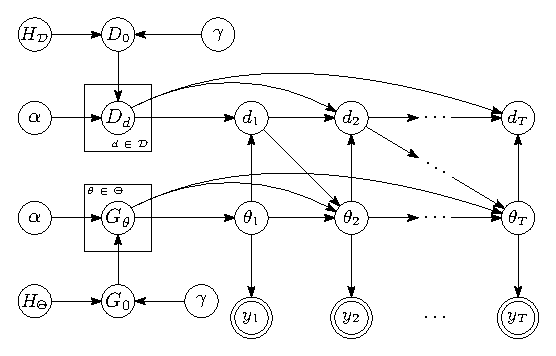
\includegraphics[width=0.4\textwidth]{figures/HDPEDHMM.eps}}\hspace{2em}
        \subfloat[Stateful IDHMM]{\includegraphics[width=0.4\textwidth]{figures/stateful-HDPEDHMM-v2.eps}}
        \caption{BNP \emph{discrete} SSMs used in this work.}
    \end{figure}
\end{frame}

%------------------------------------------------

\begin{frame}[plain,noframenumbering]
    \frametitle{Chapter IV: Synthetic experiments}
    \begin{figure}[ht!]
        \subfloat[Observations w. GT]{\includegraphics[width=.33\textwidth]{figures/PAPER-synthetic-data.pdf}}\hfill
        \subfloat[Hamming distance]{\includegraphics[width=.33\textwidth]{figures/Hamming-distance.pdf}}\hfill
        \subfloat[State cardinality]{\includegraphics[width=.33\textwidth]{figures/state-cardinality.pdf}}\hfill
        \caption{results from experiments on multivariate synthetic Gaussian observations with sequential Monte-Carlo inference. Connected bullets are median scores.}
        \textcolor{red}{*}\footnotesize{Hamming distance: the number of positions at which the corresponding symbols are different, for two sequences of equal length -- i.e. measuring the \emph{edit distance}}
    \end{figure}
\end{frame}

\begin{frame}[plain,noframenumbering]
    \frametitle{Chapter IV: Synthetic experiments}
    \begin{figure}[ht!]
        \subfloat[Duration priors]{\includegraphics[width=.33\textwidth]{figures/PAPER-duration-distributions.pdf}}\hfill
        \subfloat[Gaussian mixture duration]{\includegraphics[width=.33\textwidth]{figures/gaussian-durations.pdf}}\hfill
        \subfloat[Poisson mixture duration]{\includegraphics[width=.33\textwidth]{figures/poisson-durations.pdf}}\hfill
        \caption{results from experiments with different duration priors. Connected bullets show median scores.}
    \end{figure}
\end{frame}

%------------------------------------------------
\begin{frame}[plain,noframenumbering]
    \frametitle{Chapter IV: Conclusion and future work}
    \begin{itemize}
        \item Bayesian nonparametric state-space models show promise in this difficult domain 
        \item For sequence modelling and novelty detection, these models could make unsupervised time-series
            segmentation more interpretable 
        \item Purely as a first pass through the data, this approach allows the scientist to identify regions of interest
        \item By using a PPS we can quickly iterate over state-space models which are 
            \begin{itemize}
                \item Non I.I.D.  and which have non-geometric durations
                \item Unsupervised
                \item Nonparametric
            \end{itemize}
        \item {\bf Future work}: incorporate domain knowledge through priors, semi-supervised learning, transfer
            learning between different observation domains (e.g. different human users, or different animals in an
            animal modelling setting). 
    \end{itemize}
\end{frame}

%------------------------------------------------

\begin{frame}[plain]
    \frametitle{Reminder: Where are we now in the control hierarchy?}
    \begin{figure}
        \centering
        \includegraphics[width=0.9\textwidth]{figures/tucker.png}
        \caption{Generalised control framework for active prostheses and orthoses \citep{tucker2015control}.}
    \end{figure}
\end{frame}

%------------------------------------------------

\section{Chapter V: Gaussian process regression for prosthesis control [Translation/Execution layer]} 

\begin{frame}[plain]
    \frametitle{Chapter V: Gaussian process regression for prosthesis control [Translation/Execution layer]} 
    \begin{columns}[t] 
        \column{.5\textwidth} % Left column and width
        \fbox{
            \begin{minipage}{7cm}
                The purpose of the mid-level controller is to convert the estimated intent output 
                from the high-level controller to a device state for the low-level controller to track.
            \end{minipage}
        }
        \begin{itemize}
            \item Want to illicit smooth anthropomimetic transition between incidents (velocities) 
            \item `Locomotion envelopes' (collection of multivariate GPR vector fields) provides one way of achieving
                this goal 
            \item Transition has to be done safely i.e. with uncertainty estimates on predictions $\rightarrow$ GPs are a
                natural fit
        \end{itemize}
        \column{.5\textwidth} % Right column and width
        \vspace{-1cm}
        \begin{figure}
            \centering
            %\includegraphics[angle=0,width=.45\textwidth]{/home/nd/cloud/thesis/figures/LE-figures/prosthesis.JPG}
            \includegraphics[width=.6\textwidth]{/home/nd/cloud/thesis/figures/LE-figures/prosthesis-final2-mirrored.jpg}
            \caption{Test-bed (experimental prosthesis)}
        \end{figure}
    \end{columns}
\end{frame}

\begin{frame}[plain]
    \frametitle{Chapter V: High-level idea} 
    \begin{figure}
        \centering
        \includegraphics[width=0.8\textwidth]{/home/nd/cloud/thesis/figures/common-figures/human-robot-function-learning.eps}
        \caption{A simplified illustration of a human locomotion manifold on the left, and its
correspondent manifold, for the AAM on the right.}
    \end{figure}
    We can learn this mapping using Gaussian process regression.
\end{frame}

%------------------------------------------------

\begin{frame}[plain,noframenumbering]
    \frametitle{Chapter V: Observations for supervised learning}
    \begin{figure}
        \centering
        \includegraphics[width=0.8\textwidth]{/home/nd/cloud/thesis/figures/LE-figures/ankle-angle-trajectories-time-subject-6.pdf}
        \caption{Un-normalised ankle plantarflexion angle with $\pm$ two standard deviations, for subject 6, during normal walking at three different speeds.}
    \end{figure}
\end{frame}


%------------------------------------------------

\begin{frame}[plain,noframenumbering]
    \frametitle{Chapter V: Gaussian process regression}
    \begin{figure}[ht!]
        \subfloat[Training inputs $\mathbf{X}$ with
        targets $\mathbf{y}$.]{\includegraphics[width=.32\textwidth]{/home/nd/cloud/thesis/figures/LE-figures/heatmapTrainPlot-ID17-Right_Ankle_PlantarFlexion_Angle.eps}}
        \subfloat[Posterior predictive mean function as
        heatmap.]{\includegraphics[width=.32\textwidth]{/home/nd/cloud/thesis/figures/LE-figures/heatmapPlot-ID17-Right_Ankle_PlantarFlexion_Angle.eps}}\hfill
        \subfloat[Posterior predictive mean surface for tests
        inputs]{\includegraphics[width=.31\textwidth]{/home/nd/cloud/thesis/figures/LE-figures/manifoldPlot-ID17-Right_Ankle_PlantarFlexion_Angle.eps}}\hfill
\caption{Workflow used in obtaining an ankle plantarflexion angle regression manifold, for subject 17.}
    \end{figure}
\end{frame}

%------------------------------------------------

\begin{frame}[plain,noframenumbering]
    \frametitle{Chapter V: Stride-time regression}
    \begin{figure}[ht!]
        \subfloat[Comparative stride duration.]{\includegraphics[width=.4\textwidth]{/home/nd/cloud/thesis/figures/LE-figures/subject-10-violin-plot-duration.pdf}}
        \subfloat[Curve fitted to Arnold et al. (2013) stride
duration observations.]{\includegraphics[width=.4\textwidth]{/home/nd/cloud/thesis/figures/LE-figures/gait-cycle-time-comparisson-Arnold-2.pdf}}
\caption{Regressing across stride durations; the shaded region in (b) shows our duration domain.}
            \end{figure}
\end{frame}

%------------------------------------------------

\begin{frame}[plain,noframenumbering]
    \frametitle{Chapter V: Simulated results}
    \begin{figure}[ht!]
        \subfloat[$v=0.6$m/s.]{\includegraphics[width=.4\textwidth]{/home/nd/cloud/thesis/figures/LE-figures/v0.eps}}
        \hspace{0.5cm}
        \subfloat[$v=1.6$m/s.]{\includegraphics[width=.49\textwidth]{/home/nd/cloud/thesis/figures/LE-figures/vf.eps}}
        \caption{Panels show gait cycle simulations for velocities outside the training data.}
    \end{figure}
\end{frame}

%------------------------------------------------

\begin{frame}[plain,noframenumbering]
    \frametitle{Chapter V: Simulated results}
    \begin{figure}[ht!]
        \subfloat[Plantarflexion angle]{\includegraphics[width=.5\textwidth]{/home/nd/cloud/thesis/figures/LE-figures/subject-6-torque-v-angle.pdf}}
        \subfloat[Knee angle (sagittal plane)]{\includegraphics[width=.5\textwidth]{/home/nd/cloud/thesis/figures/LE-figures/subject-6-torque-v-angle-knee.pdf}}
        \caption{Measured and inferred ankle kinetics for subject 6. Curves are shown for velocities inside and outside the training data. Dashed curves lie on the extrema of the test points and the
experimental values for the curves of 0.8, 1.2 and 1.6m/s are shown as well.}
    \end{figure}
\end{frame}

%------------------------------------------------

\begin{frame}[plain,noframenumbering]
    \frametitle{Chapter V: Hardware results}
    \begin{figure}
        \centering
        \includegraphics[width=0.8\textwidth]{/home/nd/cloud/thesis/figures/LE-figures/mainResult-slow.pdf}
        \vspace{-1em}
        \caption{Experimental results of walking at $v=0.37$m/s} 
    \end{figure}
\end{frame}

\begin{frame}[plain,noframenumbering]
    \frametitle{Chapter V: Conclusion and future work}
    \begin{itemize}
        \item Demonstrated a robust method for smoothly (and anthropomimetically) transitioning between velocities 
        \item Hardware and simulation tests, demonstrate that for isolated test-cases the method performs well
        \item Safety is account for (though not yet implemented) due to the uncertainty quantifications inherent in GP
           construction 
        \item {\bf Future work}: 
            \begin{itemize}
                \item Implement sharing of information through coregionalised (vector output) GPs
                \item Investigate methods for most efficiently transitioning between instances (could involve DMPs)
                \item Proposition methods for conjoining (effectively sewing together) locomotion envelopes for
                    different locomotion instances (e.g. LEs for biking, LEs for walking up a staircase) 
                \item Need to develop methods which take complex noise models into account
            \end{itemize}
    \end{itemize}
\end{frame}

%------------------------------------------------

\section{Conclusion}
\begin{frame}[plain,noframenumbering]
    \frametitle{{\bf Conclusion and future work}}
    \begin{itemize}
        \item Have demonstrated and suggested various `primitives' that \emph{could} form part of
            \citet{tucker2015control}'s hierarchical control stratification
        \item Obviously lacking is an overarching (i.e. \emph{global}) system that can selectively use these primitives
            to restore locomotion to people with AAMs
        \item Proposed methods include a mix of unsupervised and supervised learning strategies, ultimately though, we
            posit that these methods will have to be predominantly unsupervised 
        \item {\bf The ultimate goal:} We envision, ideally and eventually, a system capable of merely being `put on',
            without the tedious parameter tuning, capable of establishing faithful and comfortable locomotion, which
            becomes \emph{better} with time as the system learns and adapts to its user (not unlike one-shot
            learning)
    \end{itemize}
\end{frame}


\iffalse % everything until \fi is not included in the slides
%------------------------------------------------
\begin{frame}[plain,noframenumbering]
    \frametitle{Lion ecology}

    \begin{itemize}
        \item In sequential acceleration data there is a natural dependence between observations of movement or behaviour. Most analyses are \textcolor{red}{i.d.d.} and ignore this.
        \item Analysis of acceleration data
            has been focused on identifying patterns in the observed waveforms that correspond to a known behaviour or movement mode: \textcolor{red}{parametric statistics}
        \item This requires observing the animal, manually assigning labels corresponding to behaviours to segments of the data - such \textcolor{red}{supervised learning} is often expensive and not always feasible
        \item Most work in this area has been \textcolor{red}{frequentist} in nature; significant prior domain knowledge (from zoologist) is currently not incorporated in the statistical analysis
    \end{itemize}

\end{frame}

%------------------------------------------------

\begin{frame}[plain,noframenumbering]
    \frametitle{Lions as state space models (SSM)}

    In this work, we propose to mend these four deficiencies through a new flavour of SSM which effects full

    \begin{itemize}
        \item non-IID
        \item unsupervised (though we allow for semi-supervision)
        \item Bayesian
        \item nonparametric
    \end{itemize}
    -learning.

    \begin{block}{Take home}
        This allows us to: produce a \textcolor{red}{segmentation and clustering} of \textcolor{red}{sequential} biotelemetry data, taking into account zoologists \textcolor{red}{domain knowledge}, as well as \textcolor{red}{observations}, and allowing us to not only \textcolor{red}{recognise known behaviours}, but also \textcolor{red}{discover new behaviours}.
    \end{block}

    % \begin{figure}
    %   \includegraphics[width=0.8\linewidth]{para.png}
    %   \caption{left: parametric case ; right: nonparametric case}
    % \end{figure}

\end{frame}

%------------------------------------------------

\section{State space modelling}

\subsection{Hidden Markov model}
\begin{frame}[plain,noframenumbering]
    \frametitle{State space models: Hidden Markov model}


    \begin{columns}[c] 

        \column{.5\textwidth} 

        \begin{itemize}
            \item HMMs are SSMs with discrete states
            \item HMMs have a latent Markov process that transitions between a finite number of discrete states at discrete times and is endowed with per state emission distributions.
            \item HMMs is a highly successful model in some domains, but is subject to \textcolor{red}{two} very large deficiencies
        \end{itemize}

        \column{.5\textwidth} % Right column and width

        \begin{figure}
            \includegraphics[width=1.0\linewidth]{hmm.png}
            \caption{Hidden Markov model.}
        \end{figure}

    \end{columns}

\end{frame}

%------------------------------------------------

\section{Results}
\subsection{Synthetic observations}
\begin{frame}[plain,noframenumbering]
    \frametitle{Synthetic observations}

    \begin{columns}[c] 

        \column{.5\textwidth} 

        \begin{figure}
            \includegraphics[width=1.0\linewidth]{synthetic-data-plot-data1.pdf}
            \caption{Synthetic observations one.}
        \end{figure}

        \column{.5\textwidth} % Right column and width

        \begin{figure}
            \includegraphics[width=1.0\linewidth]{synthetic-data-plot-data2.pdf}
            \caption{Synthetic observations two.}
        \end{figure}

    \end{columns}

\end{frame}

%------------------------------------------------

\begin{frame}[plain,noframenumbering]
    \frametitle{Sample latent sequences}

    \begin{columns}[c] 

        \column{.5\textwidth} 

        \begin{figure}
            \includegraphics[width=1.0\linewidth]{state-seq-data1.pdf}
            \caption{Sample latent sequences for observations set one.}
        \end{figure}

        \column{.5\textwidth} % Right column and width

        \begin{figure}
            \includegraphics[width=1.0\linewidth]{state-seq-data2.pdf}
            \caption{Sample latent sequences for observations set two.}
        \end{figure}

    \end{columns}

\end{frame}

%------------------------------------------------

\begin{frame}[plain,noframenumbering]
    \frametitle{Hamming distances}

    \begin{columns}[c] 

        \column{.5\textwidth} 

        \begin{figure}
            \includegraphics[width=1.0\linewidth]{hamming-distance-plot-data1.pdf}
            \caption{Hamming distance for observations set one.}
        \end{figure}

        \column{.5\textwidth} % Right column and width

        \begin{figure}
            \includegraphics[width=1.0\linewidth]{hamming-distance-plot-data2.pdf}
            \caption{Hamming distance for observations set two.}
        \end{figure}

    \end{columns}

\end{frame}

%------------------------------------------------

\subsection{Lion (Panthera leo) observations}
\begin{frame}[plain,noframenumbering]
    \frametitle{Lion observations}

    \begin{figure}
        \includegraphics[width=1.0\linewidth]{acc-10p-50s-again-vacar.pdf}
        \caption{Raw tri-axial acceleration observations.}
    \end{figure}


\end{frame}

%------------------------------------------------


\section{Anglican queries}
\begin{frame}[plain,noframenumbering]
    \frametitle{Anglican queries}

    \begin{itemize}
        \item HDP implementation
        \item mixtures
        \item inference (SMC inference, particles and samples)
            % \item \textit{other state space models}
    \end{itemize}

\end{frame}


\fi

%------------------------------------------------

\begin{frame}[plain,noframenumbering]
    \begin{figure}
        \includegraphics[width=0.5\linewidth]{figures/lion.eps}
    \end{figure}
    \Huge{\centerline{Questions?}}
\end{frame}

%----------------------------------------------------------------------------------------

\begin{frame}[plain,noframenumbering]
    \frametitle{References}
    \footnotesize
    \bibliographystyle{plainnat}
    \nocite{*}
    \bibliography{talk}
\end{frame}

%------------------------------------------------

\begin{frame}[plain]
    \frametitle{Understanding animal behaviour from observations} 
    \begin{columns}[t] % The "c" option specifies centered vertical alignment while the "t" option is used for top vertical alignment

        \column{.5\textwidth} % Left column and width

        \begin{itemize}
            \small
        \item Oxford's zoologists have been tracking prides of lions for years 
        \item Famous members include Cecil and Xanda (killed by trophy hunters in July, two years after Cecil)
        \item Observations $(y \in \mathbb{R}^d, d\gg1)$ often sampled at years at a time, sometimes at very high frequencies 
        \item Use of especially accelerometry is widespread within biotelemetry as a means of measuring an animal’s activity quantitatively
        \item Biotelemetry is used as a means of classifying behaviour i.e. to \emph{understand} their ecology
            %\item Animal accelerometer data allow ecologists to identify correlates and drivers of behaviour
            %\item Use of accelerometers is widespread within biotelemetry as a means of measuring an animal’s activity quantitatively
            %\item Recordings are sampled at a high temporal resolution, sometimes for years at a time, resulting in terabytes of data
    \end{itemize}

    \column{.5\textwidth} % Right column and width
    \vspace{-2em}
    \begin{figure}[ht]
        \subfloat[Puma. Not lion. Still has collar, so we're ok.]{\includegraphics[width=1.\textwidth]{figures/puma1.jpg}}\\[-0em]
        \subfloat[Collared lions]{\includegraphics[width=1.\textwidth]{figures/lionCollar.jpg}}
    \end{figure}
\end{columns}
    \end{frame}


    \begin{frame}[plain,noframenumbering]
        \frametitle{Labelling lion observations}
        \begin{figure}[ht!]
            \includegraphics[width=0.92\linewidth]{figures/PAPER-main-result.eps}
            \vspace{-0.5em}
            \caption{{\bf top} --  signal, {\bf middle} -- state sequences inferred by models through unsupervised learning and {\bf bottom} -- manually labelled fuzzy ground truth state sequence}
        \end{figure}
    \end{frame}


    \begin{frame}[plain,noframenumbering]
        \frametitle{Detailed analysis: a hunt}
        \begin{figure}
            \includegraphics[width=0.9\linewidth]{figures/new-main-plot.pdf}
            \caption{{\bf first two panels} -- signal and ground truth; {\bf next two panels} -- zoomed in; {\bf final two panels} --  assigned detailed labelling by IDHMM and stateful IDHMM as established by listening to audio, ``concluding'' that models learned \emph{meaningful} new behaviours.}
        \end{figure}
    \end{frame}


    \end{document} 
